%-------------------------------------------------------------------------------
%   PACKAGES AND OTHER DOCUMENT CONFIGURATIONS
%-------------------------------------------------------------------------------
\documentclass[paper=a4, fontsize=11pt]{scrartcl} % A4 paper and 11pt font size
\usepackage{fancyhdr} % Required for custom headers
\usepackage{lastpage} % Required to determine the last page for the footer
\usepackage{extramarks} % Required for headers and footers
\usepackage[usenames,dvipsnames]{color} % Required for custom colors
\usepackage{graphicx} % Required to insert images
\usepackage{listings} % Required for insertion of code
\usepackage{courier} % Required for the courier font
\usepackage[T1]{fontenc} % Use 8-bit encoding that has 256 glyphs
\usepackage[english]{babel} % English language/hyphenation
\usepackage{amsmath,amsfonts,amsthm} % Math packages
\usepackage{enumitem}
\usepackage{algorithm}
\usepackage{algpseudocode}

\usepackage{sectsty} % Allows customizing section commands
\allsectionsfont{\centering \normalfont\scshape} % Make all sections centered, 
                                                 % the default font and small 
                                                 % caps

\pagestyle{fancyplain} % Makes all pages in the document conform to the custom
                       % headers and footers
\fancyhead{} % No page header - if you want one, create it in the same way as 
             % the footers below
\fancyfoot[L]{} % Empty left footer
\fancyfoot[C]{} % Empty center footer
\fancyfoot[R]{\thepage} % Page numbering for right footer
\renewcommand{\headrulewidth}{0pt} % Remove header underlines
\renewcommand{\footrulewidth}{0pt} % Remove footer underlines
\setlength{\headheight}{13.6pt} % Customize the height of the header

\numberwithin{equation}{section} % Number equations within sections (i.e. 1.1, 
                                 % 1.2, 2.1, 2.2 instead of 1, 2, 3, 4)
\numberwithin{figure}{section} % Number figures within sections (i.e. 1.1, 1.2,
                               % 2.1, 2.2 instead of 1, 2, 3, 4)
\numberwithin{table}{section} % Number tables within sections (i.e. 1.1, 1.2, 
                              % 2.1, 2.2 instead of 1, 2, 3, 4)

\setlength\parindent{0pt} % Removes all indentation from paragraphs - comment 
                          % this line for an assignment with lots of text

%-------------------------------------------------------------------------------
%   TITLE SECTION
%-------------------------------------------------------------------------------

\newcommand{\horrule}[1]{\rule{\linewidth}{#1}} % horizontal cmd, arg = height
\newcommand{\name}{Colin Bradford} % student name
\newcommand{\hwnum}{1} % homework number
\newcommand{\classnum}{CS 325} % class num with abreviation
\newcommand{\classname}{Analysis of Algorithms} % name of class
\newcommand{\hwtitle}{\classnum: Project \hwnum}

\title{ 
    \normalfont \normalsize 
    \textsc{Oregon State University} \\ [25pt]
    \large Project Group 21
    \horrule{0.5pt} \\[0.4cm] % Thin top horizontal rule
    \huge \hwtitle \\ % The assignment title
    \horrule{2pt} \\[0.5cm] % Thick bottom horizontal rule
}

\author{
    Colin Bradford
    \and
    Charles Jenkins
    \and
    Albert Le
} % Your name

\date{\normalsize\today} % Today's date or a custom date

%-------------------------------------------------------------------------------
%   DOCUMENT
%-------------------------------------------------------------------------------
\begin{document}

\maketitle % Print the title


\section{Theoretical Run-time Analysis}
\begin{enumerate}[label=\bfseries Algorithm \arabic*:]
    % Algo 1
    \item \hfill \\
    \begin{description}
        \item[Pseudo-code] \hfill \\
        \begin{algorithmc}
            \caption{Algorithm 1: Enumeration}
            \Require{$A$ is an $n$-sized array of small integers.}
            \Function{Max-Subarray}{$A$}
                \State $n \gets A$.size
                \State $maxSum \gets$ null
                \State $curSum \gets 0$
                \State $start \gets 0$
                \State $end \gets 0$
                \For{$i \gets 0 \textrm{ to } n$}
                    \For{$j \gets i \textrm{ to } n$}
                        \State $curSum \gets 0$
                        \For{$k \gets i \textrm{ to } j$}
                            \State $curSum \gets curSum + A[k]$
                        \EndFor
                        \If{$curSum > maxSum$}
                            \State $maxSum \gets curSum$
                            \State $start \gets i$
                            \State $end \gets j$
                        \EndIf
                    \EndFor
                \EndFor
                \State \Return $A[start..end]$
            \EndFunction
        \end{algorithmc}
        \item[Run-time Analysis] \hfill \\
        Based on the pseudo-code we can conclude that the equation for 
        time complexity can be given by
        \[ T(n) = T(n - 1) + T_1(n) \]
        \[ T_1(n) = T_1(n - 1) + T_2(n) \]
        \[ T_2(n) = T_2(n - 1) + c \]
        We can reduce both $T_1(n)$ and $T_2(n)$ to their time complexities
        and then finally $T(n)$
        \begin{align*}
            T_2(n - 1) & = T_2(n - 2) + c \\
            \ldots & = c + c + c + \ldots + c \\
            T_2(n) & = nc
        \end{align*}
        Therefore $T_2(n) = \Theta(n)$.
        \begin{align*}
            T_1(n - 1) & = T_2(n - 2) + \Theta(n) \\
            \ldots & = \Theta(n) + \Theta(n) + \Theta(n) + \ldots + \Theta(n) \\
            T_1(n) & = n\Theta(n)
        \end{align*}
        Therefore $T_1(n) = \Theta(n^2)$.
        \begin{align*}
            T(n - 1) & = T(n - 2) + \Theta(n^2) \\
            \ldots & = \Theta(n^2) + \Theta(n^2) + \Theta(n^2) + \ldots + \Theta(n^2) \\
            T(n) & = n\Theta(n^2)
        \end{align*}
        Therefore $T(n) = \Theta(n^3)$.
    \end{description}

    % Algo 2
    \item \hfill \\
    \begin{description}
        \item[Pseudo-code] \hfill \\
        \begin{algorithmc}
            \caption{Algorithm 2: Better Enumeration}
            \Require{$A$ is an $n$-sized array of small integers.}
            \Function{Max-Subarray}{$A$}
                \State $n \gets A$.size
                \State $maxSum \gets$ null
                \State $curSum \gets 0$
                \State $start \gets 0$
                \State $end \gets 0$
                \For{$i \gets 0 \textrm{ to } n$}
                    \State $curSum \gets 0$
                    \For{$j \gets i \textrm{ to } n$}
                        \State $curSum \gets curSum + A[j]$
                        \If{$curSum > maxSum$}
                            \State $maxSum \gets curSum$
                            \State $start \gets i$
                            \State $end \gets j$
                        \EndIf
                    \EndFor
                \EndFor
                \State \Return $A[start..end]$
            \EndFunction
        \end{algorithmc}
        \item[Run-time Analysis] \hfill \\
        Based on the pseudo-code we can conclude that the equation for 
        time complexity can be given by
        \[ T(n) = T(n - 1) + T_1(n) \]
        \[ T_1(n) = T_1(n - 1) + c \]
        We can reduce $T_1(n)$ to its time complexities and then finally $T(n)$
        \begin{align*}
            T_1(n - 1) & = T_1(n - 2) + c \\
            \ldots & = c + c + c + \ldots + c \\
            T_1(n) & = nc
        \end{align*}
        Therefore $T_1(n) = \Theta(n)$.
        \begin{align*}
            T(n - 1) & = T(n - 2) + \Theta(n) \\
            \ldots & = \Theta(n) + \Theta(n) + \Theta(n) + \ldots + \Theta(n) \\
            T(n) & = n\Theta(n)
        \end{align*}
        Therefore $T(n) = \Theta(n^2)$.
    \end{description}

    % Algo 3
    \item \hfill \\
    \begin{description}
        \item[Pseudo-code] \hfill \\
        \begin{algorithmc}
            \caption{Algorithm 3: Divide and Conquer}
            \Require{$A$ is an $n$-sized array of small integers.}
            \Function{Max-Subarray}{$A$}
                \State $n \gets A$.size
                \State $maxSum \gets$ null
                \State $curSum \gets 0$
                \State $mid \gets n / 2$
                \For{$i \gets 0 \textrm{ to } mid$}
                    $curSum \gets curSum + A[i]$
                \EndFor
                \For{$i \gets 0 \textrm{ to } mid$}
                    \For{$j \gets mid + 1 \textrm{ to } n$}
                        \State $curSum \gets curSum + A[j]$
                        \If{$curSum > maxSum$}
                            \State $maxSum \gets curSum$
                            \State $start \gets i$
                            \State $end \gets j$
                        \EndIf
                    \EndFor
                    \State $curSum \gets curSum - A[i]$
                \EndFor
                \State $maxArray \gets A[start..end]$
                \State $leftArray \gets$ \Call{Max-Subarray}{$A[0..mid]$}
                \State $rightArray \gets$ \Call{Max-Subarray}{$A[mid + 1..n]$}
                \If{\Call{Sum}{$leftArray$}$> maxSum$}
                    \State $maxArray \gets leftArray$
                \EndIf
                \If{\Call{Sum}{$rightArray$}$ > maxSum$}
                    \State $maxArray \gets rightArray$
                \EndIf
                \State \Return{$maxArray$}
            \EndFunction
            \Function{Sum}{$A$}
                \State $n \gets A$.size
                \State $sum \gets 0$
                \For{$i \gets 0 \textrm{ to } n$}
                    \State $sum \gets sum + A[i]$
                \EndFor
                \State \Return{$sum$}
            \EndFunction
        \end{algorithmc}
        \item[Run-time Analysis] \hfill \\
        Based on the pseudo-code we can conclude that the equation for 
        time complexity can be given by
        \[ T(n) = 2T(n/2) + n \]
        Let $n = 2^k$
        \begin{align*}
            T(n/2) & = 2T(n/4) + n/2 \\
            \ldots & = n + 2(n/2 + 2(n/4 + 2(\ldots))) \\
            T(n) & = n\lg{n} + n
        \end{align*}
        Therefore $T(n) = \Theta(n\lg{n})$
    \end{description}

    % Algo 4
    \item \hfill \\
    \begin{description}
        \item[Pseudo-code] \hfill \\
        \begin{algorithmc}
            \caption{Max-Subarray finds the subarray with the max sum of all its elements}
            \Require{$A$ is an $n$-sized array of small integers.}
            \Function{Max-Subarray}{$A$}
                \State $n \gets A$.size
                \State $maxSum \gets null$
                \State $curSum \gets 0$
                \State $curStart \gets 0$
                \State $start \gets 0$
                \State $end \gets 0$
                \For{$i \gets 0 \textrm{ to } n$}
                    \State $curSum \gets curSum + A[i]$
                    \If{$curSum < 0$}
                        \State $curSum \gets 0$
                        \State $curStart \gets i + 1$
                    \EndIf
                    \If{$curSum > maxSum$}
                        \State $maxSum \gets curSum$
                        \State $end \gets i + 1$
                        \State $start \gets curStart$
                    \EndIf
                \EndFor
                \State \Return $A[start..end]$
            \EndFunction
        \end{algorithmc}
        \item[Run-time Analysis] \hfill \\
        Based on the pseudo-code we can conclude that the equation for 
        time complexity can be given by
        \[ T(n) = T(n - 1) + c \]
        \begin{align*}
            T(n - 1) & = T(n - 2) + c \\
            \ldots & = c + c + c + \ldots + c \\
            T(n) & = nc
        \end{align*}
        Therefore $T(n) = \Theta(n)$.
    \end{description}
\end{enumerate}

\section{Proof of Correctness (Algorithm 3)}
\begin{proof}
    The loop returns the sum of all elements $A[1]$ through $A[n]$. \\
    Let our loop invariant be: $S = $ sum of the first $k$ elements of $A$. \\
    \underline{Initialization:} before for the loop starts,
    $k = 0$ and $S = 0$, which satisfies our loop invariant trivially as
    the sum of 0 elements is 0. \\
    \underline{Maintenance:} Assume after a loop that $S$ will be equal to
    the sum of the first $k + 1$ elements of $A$. Let $S$ be the sum of the 
    first $k$ elements of $A$ before the loop. After the loop we have 
    $S \gets S + A[k + 1]$. The loop invariant holds for Maintenance. \\
    \underline{Termination:} The loop terminates when $k = n$. Since we know
    that $S$ is the sum of the first $k$ elements, and $k = n$, then we can 
    say that $S$ is the sum of the first $n$ elements. Thus we have proven the claim. \\
    In addition we know that when the loop terminates, the maximum subarray will
    be described by $A[start..end]$ which is maintained throughout the loop.
\end{proof}
\begin{proof}
    \underline{Base Case $n = 1$} \\
    Trivial as the max subarray of an array of size 1 will be itself. \\
    \underline{Inductive Case} \\
    Assume Max-Subarray correctly returns the max subarray for all arrays
    for 1 through $k$. \\
    Let $A$ be an array with size $n$ \\
    Let $n = 2^{k + 1}$ \\
    We can see that there are two Max-Subarray calls each with a subarray of
    size $n/2$. Thus we can say that these calls are made with subarrays of
    size $2^k$ as $2^{k + 1} / 2 = 2^k$. Thus based on our assumptions they 
    will return the max subarray. \\
    In the proof above, we have proven that for any array of size $n$ the 
    array will find the max subarray. Thus when we find the max of each the left,
    right and middle subarrays, we will return the max subarray. Thus the algorithm
    returns correctly.
\end{proof}


\section{Testing}
Testing was automated to read in test sets from files such as 
MSS\_TestSetsSp15.txt and check our solutions against them. A variety of test 
cases were used to explore cases of arrays that were long, short, 
predominately negative, predominately positive, palindromic, ending with 
an empty subarray, containing a single value, etc. All our test cases
passed for all four algorithms.

\section{Experimental Analysis}
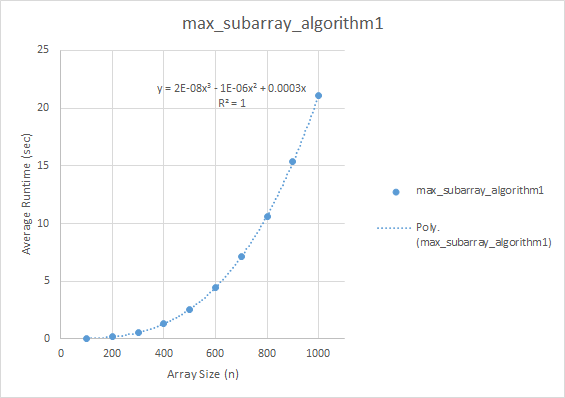
\includegraphics[width=\textwidth]{algo1Plot}
\includegraphics[width=\textwidth]{alg1_table}
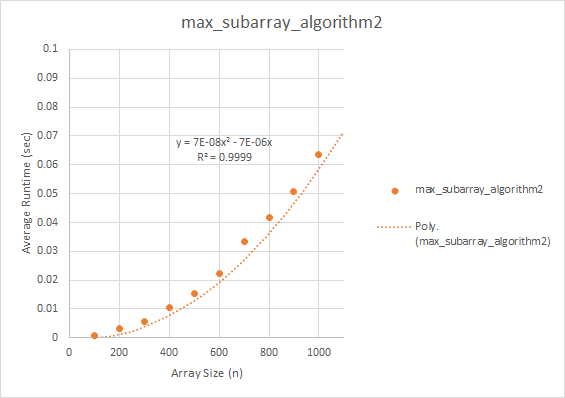
\includegraphics[width=\textwidth]{algo2Plot}
\includegraphics[width=\textwidth]{alg2_table}
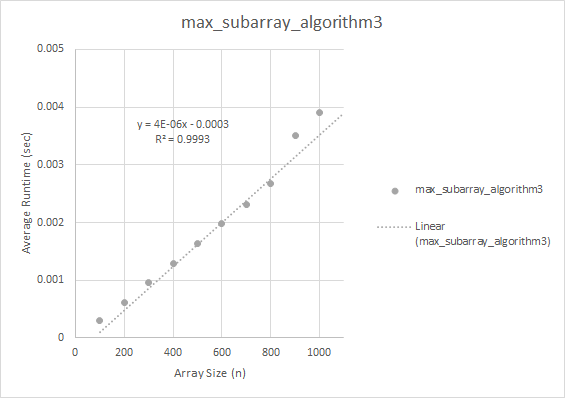
\includegraphics[width=\textwidth]{algo3Plot}
\includegraphics[width=\textwidth]{alg3_table}
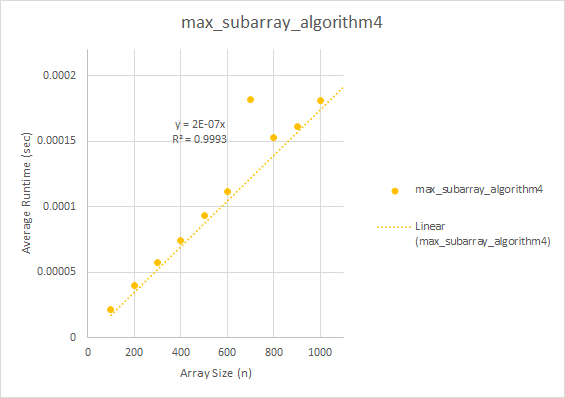
\includegraphics[width=\textwidth]{algo4Plot}
\includegraphics[width=\textwidth]{alg4_table}
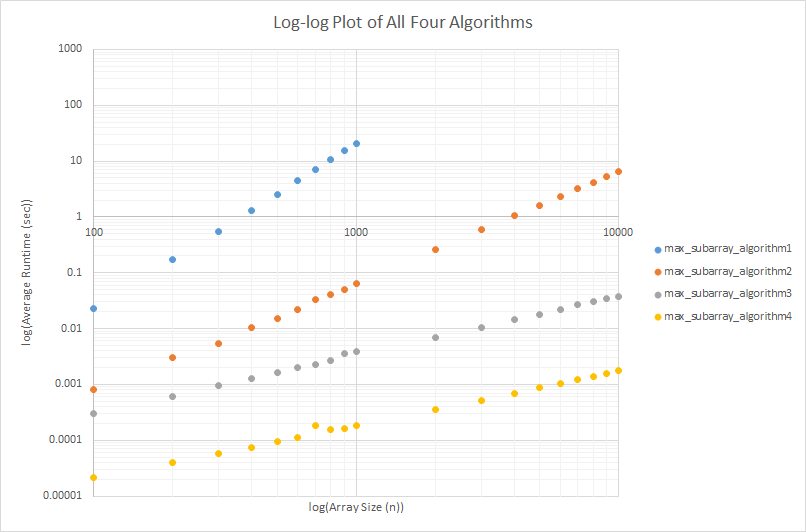
\includegraphics[width=\textwidth]{all4Plot}


\section{Extrapolation and Interpretation}
% Example of how to include a graphic below
% 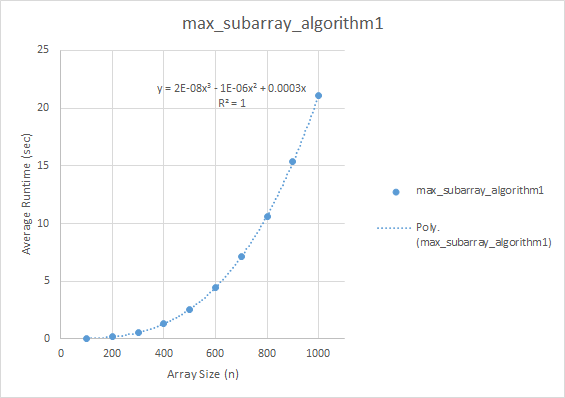
\includegraphics[width=\textwidth]{algo1Plot}
\begin{description}
    % Algo 1
    \item[Algorithm 1] \hfill \\
    \begin{description}
        \item[Experimental Run-time Function] $f(n) = 2E^{-08}n^3 - 1E^{-06}n^2 + 0.0003n$ This matches our theoretical runtime of $\Theta(n^3)$. \\
        \item[Biggest n in an hour] In one hour the biggest solvable instance is: 3600 sec = $2E^{-08}n^3$ - $1E^{-06}n^2 + 0.0003n$ --> $n = 5646$ \\
    \end{description}

    % Algo 2
    \item[Algorithm 2] \hfill \\
    \begin{description}
        \item[Experimental Run-time Function] $f(n) = 7E^{-08}n^2 - 7E^{-06}n$  This matches our theoretical runtime of $\Theta(n^2)$. \\
        \item[Biggest n in an hour] In one hour the biggest solvable instance is: 3600 sec = $7E^{-08}n^2 - 7E^{-06}n$ --> $n = 226829$ \\
    \end{description}

    % Algo 3
    \item[Algorithm 3] \hfill \\
    \begin{description}
        \item[Experimental Run-time Function] $f(n) = 4E^{-06}n - 0.0003$  Our experimental data gave us
        what looks to be a linear trend line leading to the above equation. Our theoretical runtime 
        should be $\Theta(n\log{n})$. We may not have increased n enough to see this type of asymptotic behavior.
        The one-hour calculation below assumes the experimental linear equation above, however, 
        given a more accurate nlogn function, the number would be expected to be much lower. \\
        \item[Biggest n in an hour] In one hour the biggest solvable instance is: 3600 sec = $4E^{-06}n - 0.0003$ --> $n = 900000075$ \\
    \end{description}

    % Algo 4
    \item[Algorithm 4] \hfill \\
    \begin{description}
        \item[Experimental Run-time Function]  $f(n) = 2E^{-07}n$ This matches our theoretical runtime of O(n). \\
        \item[Biggest n in an hour] In one hour the biggest solvable instance is: 3600 sec = $2E^{-07}n$ --> $n = 18000000000$ \\
    \end{description}
\end{description}
\end{document}
%-------------------------------------------------------------------------------


